\chapter{Metodologia}

Neste capítulo, será mostrado a metodologia de desenvolvimento e de TCC proposto neste trabalho. O capítulo está dividido
em seções que estão disposta da seguinte maneira: na seção 3.1 será mostrado a métodologia do TCC1 e TCC2 e como ela foi
aplicada e na seção 3.2 será mostrado todo o processo de desenvolvimento do software de uma forma generica.

\section{Metodologia do TCC}

Para o desenvolvimento do trabalho de conclusão de curso, foi definido o seguinte processo da figura \ref{fig:tcc}

\begin{figure}[h!]
  \centering
  \includegraphics[keepaspectratio=true,scale=0.4]{figuras/tcc.eps}
  \caption[Processo do TCC.]{Processo do TCC. Fonte: Autor}
  \label{fig:tcc}
\end{figure}


O processo foi dividido em dois grandes marcos: O primeiro é o planejamento da ferramenta e o segundo é a execução e
resultados da aplicação de tudo que foi planejado, ou seja, é a entrega do produto, porém de acordo com a metodologia
ágil utilizada o segundo marco se iniciará junto com o primeiro.

\subsection{Marco 1: Trabalho de Conclusão de Curso 1}

O TCC se iniciou com a definição do tema do trabalho, ao definir o tema foi selecionado materiais de estudo e pesquisa
como artigos, livros, sites e outras referências importantes para elaborar o embasamento teórico do projeto. Assim que
se teve uma boa base de conteúdo foi definido o escopo do trabalho, restringindo o que será abordado e o que será
descartado.

Com o escopo bem definido se iniciou a escrita do trabalho. Em paralelo foi definido a metodologia do TCC e a
metodologia de desenvolvimento, além de documentar todos os processos que foram realizados dentro dessas metodologias; o
referencial teórico que serviu de base para o andamento do projeto; a proposta de trabalho que deu uma visão geral do
que é o software. O processo de desenvolvimento foi realizado em paralelo com toda a metodologia do TCC.

Em seguida foi elaborado a conclusão do trabalho (TCC1) e uma verificação geral no documento, ou seja, melhorar alguns
conteúdos, ortografia, gramática e outros erros encontrados. Com isso foi elaborado os slides da apresentação do TCC 1
finalizando o marco 1 do projeto.

Em concordância com o processo de condução do TCC1 foi elaborado o cronograma da figura \ref{fig:cronograma_tcc1}:

\begin{figure}[!ht]
  \centering
  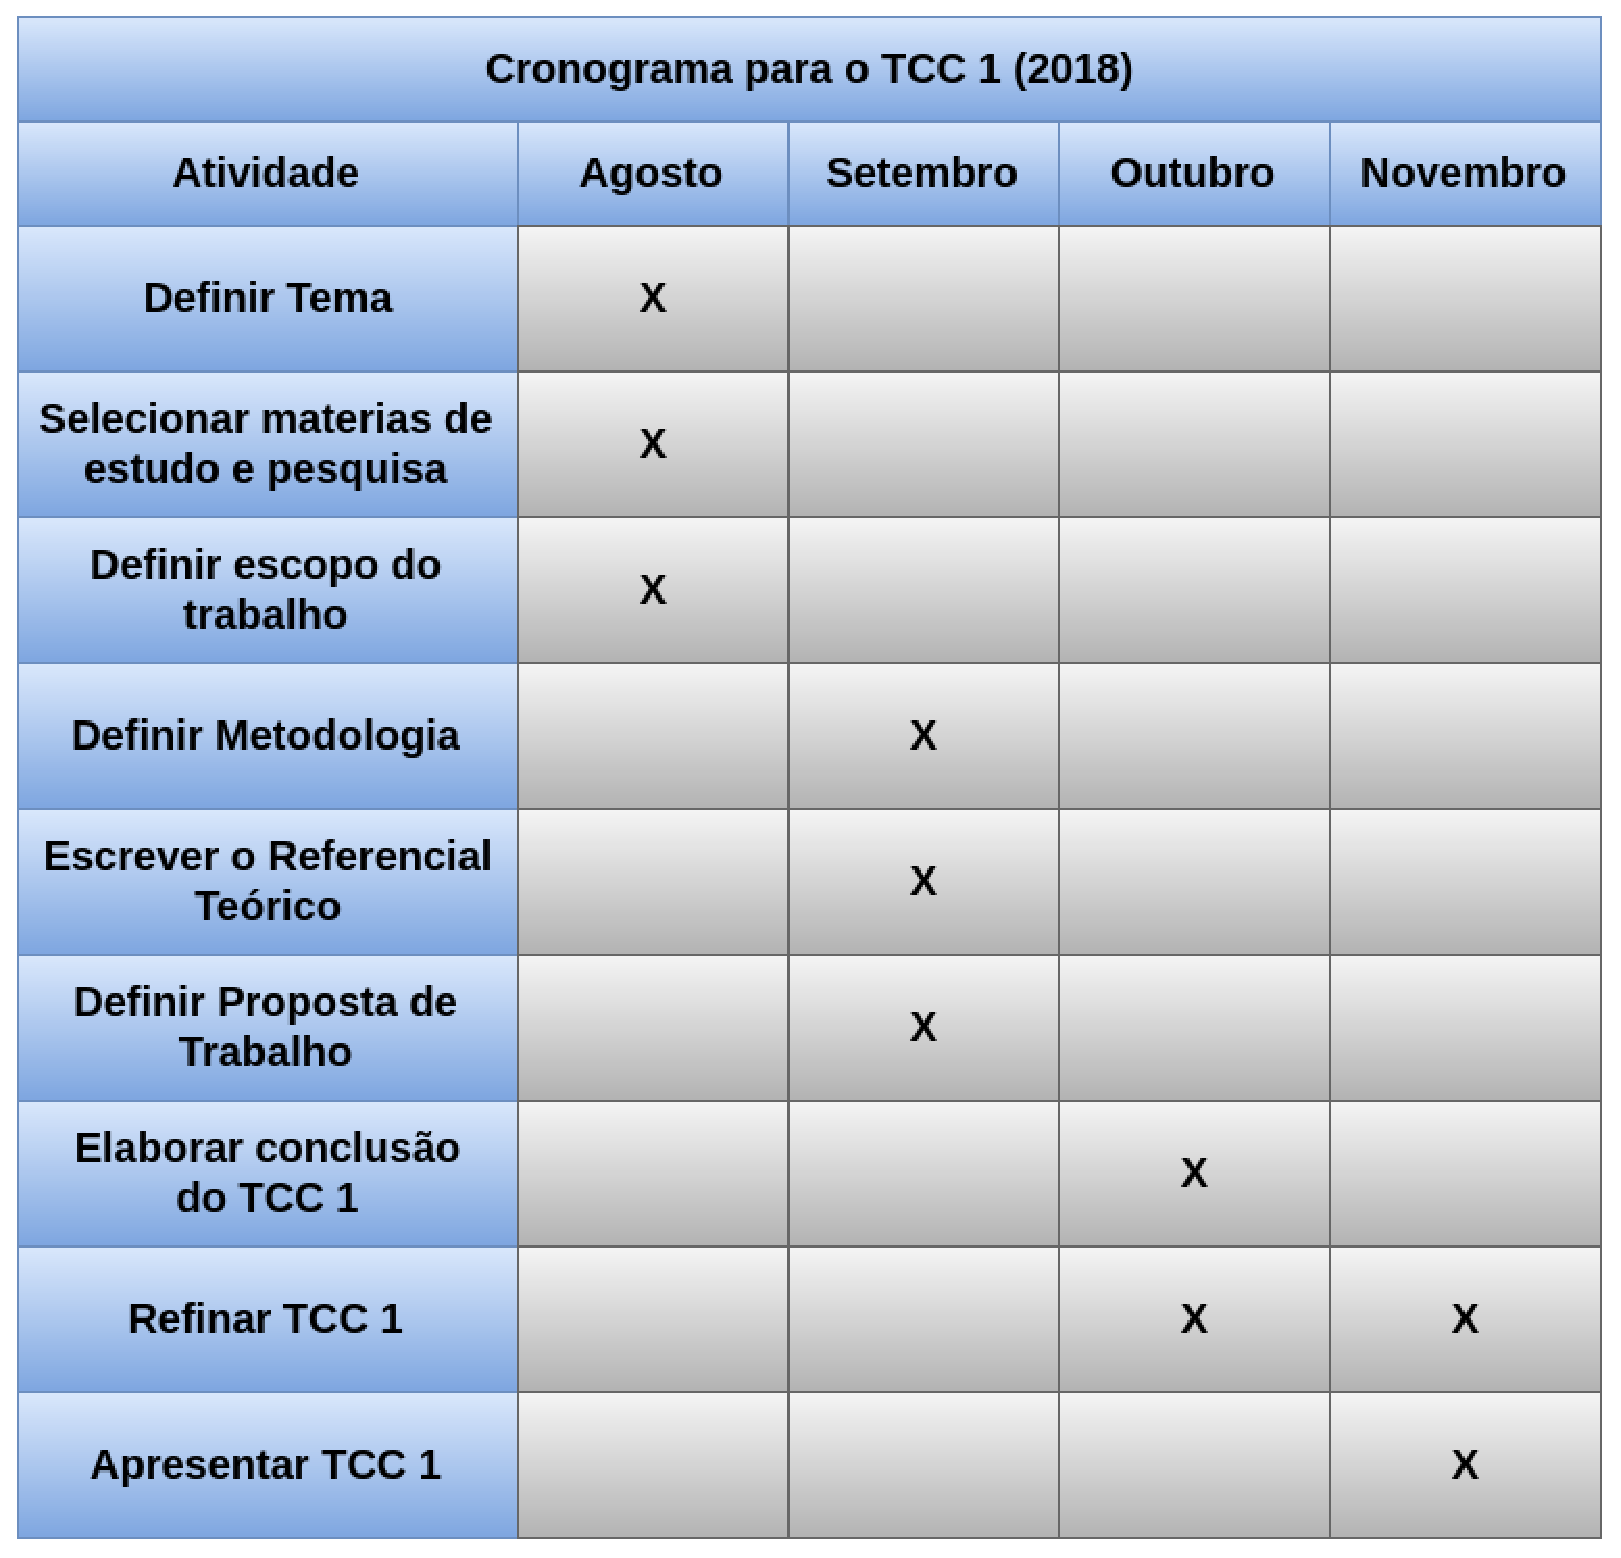
\includegraphics[keepaspectratio=true,scale=0.4]{figuras/cronograma_tcc1.eps}
  \caption[Cronograma do TCC 1.]{Cronograma do TCC 1. Fonte: Autor}
  \label{fig:cronograma_tcc1}
\end{figure}

\subsection{Marco 2: Trabalho de Conclusão de Curso 2}

Dando entrada no marco 2 do projeto foi feito os ajustes necessários do TCC 1 para o trabalho de conclusão de curso 2
ou TCC 2. Com isso foi documentado de forma sucinta os resultados da metodologia aplicada no processo de
desenvolvimento. E em paralelo foi documentado os resultados do software e sua aplicação em um contexto real.

Com os resultados documentados foi elaborado a conclusão do TCC 2 e feito uma verificação geral no
documento para melhorá-lo. Com o trabalho pronto, foi criado os slides da apresentação do TCC 2 e
assim foi finalizado o marco 2 do projeto.

Em concordância com o processo de condução do TCC2 foi elaborado o cronograma da figura \ref{fig:cronograma_tcc2}:

\begin{figure}[h!]
  \centering
  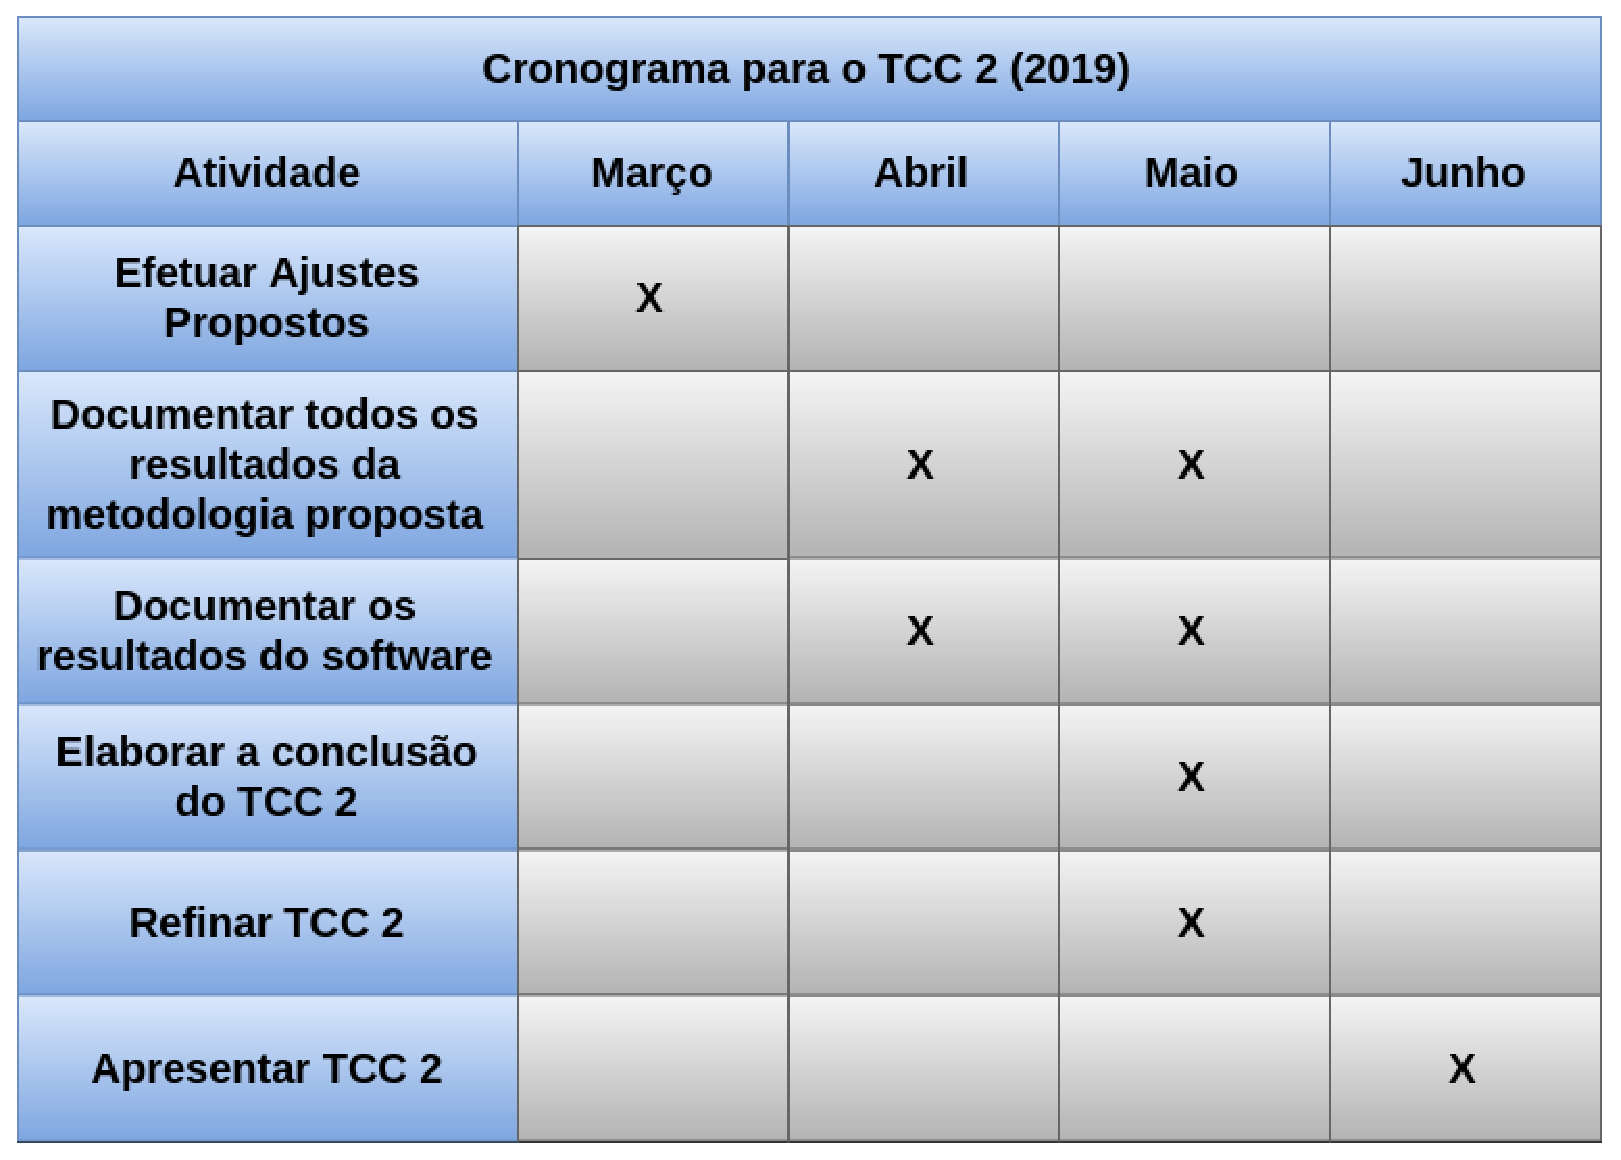
\includegraphics[keepaspectratio=true,scale=0.4]{figuras/cronograma_tcc2.eps}
  \caption[Cronograma do TCC 2.]{Cronograma do TCC 2. Fonte: Autor}
  \label{fig:cronograma_tcc2}
\end{figure}

\section{Metodologia de Desenvolvimento}

Para se construir um software é necessário seguir uma série de passos previsíveis, esses passos estão definidos no processo de software. De acordo com \cite{pressman} um processo de software pode ser visto como um conjunto de atividades, métodos, práticas e transformações que guiam pessoas na produção de software.

Para a construção do processo há uma adaptação em 3 principais níveis de acordo com o \cite{safe} (portfólio, programa e time):

\begin{itemize}
  \item O nível de portfólio foi utilizado para gerar boa parte da documentação do projeto aplicando as 3 atividades principais da engenharia de requisitos, que são elicitação, modelagem e análise;
  \item O nível de programa tem como artefatos o documento de arquitetura, as ferramentas de UX e o product backlog com sua rastreabilidade;
  \item O nível de time que é onde codificar a solução, está dividido em desenvolvimento que executa a sprint e gestão na qual aplica as práticas do scrum, além da infraestrutura e dos testes.
\end{itemize}

A construção do software foi feito seguindo uma adaptação das metodologias ágeis SCRUM, XP e SAFe para aumentar a
produtividade e eficiência do mesmo, já que o projeto todo foi realizado por uma única pessoa, ou seja, teve toda uma adaptação para isso.

Foi decidido o SCRUM devido a grande familiaridade que o desenvolvedor tem com a metodologia, ela é bastante utilizada no mercado e muito útil para organização, controle e gerenciamento do projeto. O XP também já é bem utilizado e conhecido por ser uma metodologia de desenvolvimento de software que ajuda a criar sistemas de melhor qualidade e o SAFe, este é bastante útil para padronizar o processo de forma organizada.

Para a execução, foi realizado algumas adaptações:

\begin{itemize}
  \item \textbf{Papeis}: A metodologia apresenta alguns papéis que devem ser focados pela equipe, porém como o projeto foi todo realizado por um único membro os papéis são todos realizados pelo mesmo.
  \item \textbf{SCRUM}: O SCRUM tem alguns rituais como o daily que para um único membro não se torna necessária.  Rituais como retrospectiva e revisão não foram feitas de acordo com a metodologia, pois os interessados no projeto não tem muito tempo para realizar com frequência esses rituais, porém foi feito em forma de texto e documentado na wiki do projeto.
  \item \textbf{XP}: Uma das práticas citadas do XP que não foi utilizada é a programação pareada.
  \item \textbf{SAFe}: Do SAFe foi aproveitado somente os padrões de organização do processo em níveis e a rastreabilidade dos requisitos.
  \item \textbf{Verificação e validação}: No contexto de verificação e validação foi aplicado apenas as técnicas dinâmicas, ou seja, os testes. Os testes unitários e de integração foram automatizados e foi baseados em técnicas caixa preta, particionamento de equivalência e análise de valor limite para a construção dos códigos de teste, já os testes de sistema foi realizado manualmente, entre eles temos: documentação, treinamento, teste de aceitação e teste de instalação.
  \item \textbf{Medição e Análise - GQM}: Para o GQM foi coletado métricas de código, para verificar a qualidade do mesmo, tendo como objetivo a manutenabilidade e uma métrica de equipe para verificar a evolução do conhecimento do desenvolvedor durante o projeto.
  \item \textbf{DevOps}: O DevOps tem como foco a automação de algumas atividades necessárias para agilizar e entregar código de qualidade. Entre as atividades as que foram automatizadas são: testes, ambientes e infraestrutura de instalação, coleta de algumas métricas, integração contínua e deploy.
  \item \textbf{Software Livre}: A licença escolhida para o software é a General Public License (GPL) versão 3, pois ela é a que melhor se encaixa no contexto Open Source em relação as liberdades especificadas.
\end{itemize}

O gerenciamento da sprint foi feito por quadros Kanban, na qual teremos nove quadros principais. Esses quadros se encontram nos Boards do github, utilizando como base o plugin chamado \href{https://www.zenhub.com/}{zenhub}. Para instalar é só baixar o plugin e instalar no navegador, a partir daí já conseguirá ver toda organização das issues do projeto a partir da ferramenta. Os quadros são:

\begin{itemize}
  \item \textbf{Épicos}: Épicos do software.
  \item \textbf{Features e Enables}: \textit{Features} e \textit{Enables} do software.
  \item \textbf{Novas Issues}: Novas histórias de usuário, bug reports ou qualquer tipo de situações de trabalho relacionadas ao desenvolvimento da aplicação que ainda não foram mapeadas, pontuadas ou priorizadas e consequentemente alocadas nos demais quadros.
  \item \textbf{Product Backlog}: \textit{Board} para histórias/tarefas ou correções já mapeadas e priorizadas. É importante esclarecer que nesse quadro, a prioridade é definida pela posição da \textit{issue} na \textit{board}, sendo que as posições superiores determinam maior relevância para o projeto.
  \item \textbf{Sprint Backlog}: \textit{Issues} alocadas para os desenvolvedores na \textit{sprint} corrente ou \textit{bug fixes} de alta prioridade.
  \item \textbf{Congeladas}: Issues congeladas por dependência de outras, por alguma necessidade de reavaliação da necessidade ou do esforço necessário para concluí-la, por dependência de funcionalidades externas que não são disponibilizadas pelos mantenedores, por temporária incapacidade da equipe de solucionar determinado problema, etc.
  \item \textbf{Revisão}: Tarefas concluídas que necessitam de revisão para entrarem na aplicação.
  \item \textbf{Feitas}: Código já revisado que pode ser anexado a aplicação na próxima release.
  \item \textbf{Closed}: \textit{Issues} fechadas já anexado a aplicação.
\end{itemize}

Na figura \ref{fig:desenvolvimento} está definido o processo de desenvolvimento que está no nível de programa e time.

\begin{figure}[h!]
	\centering
  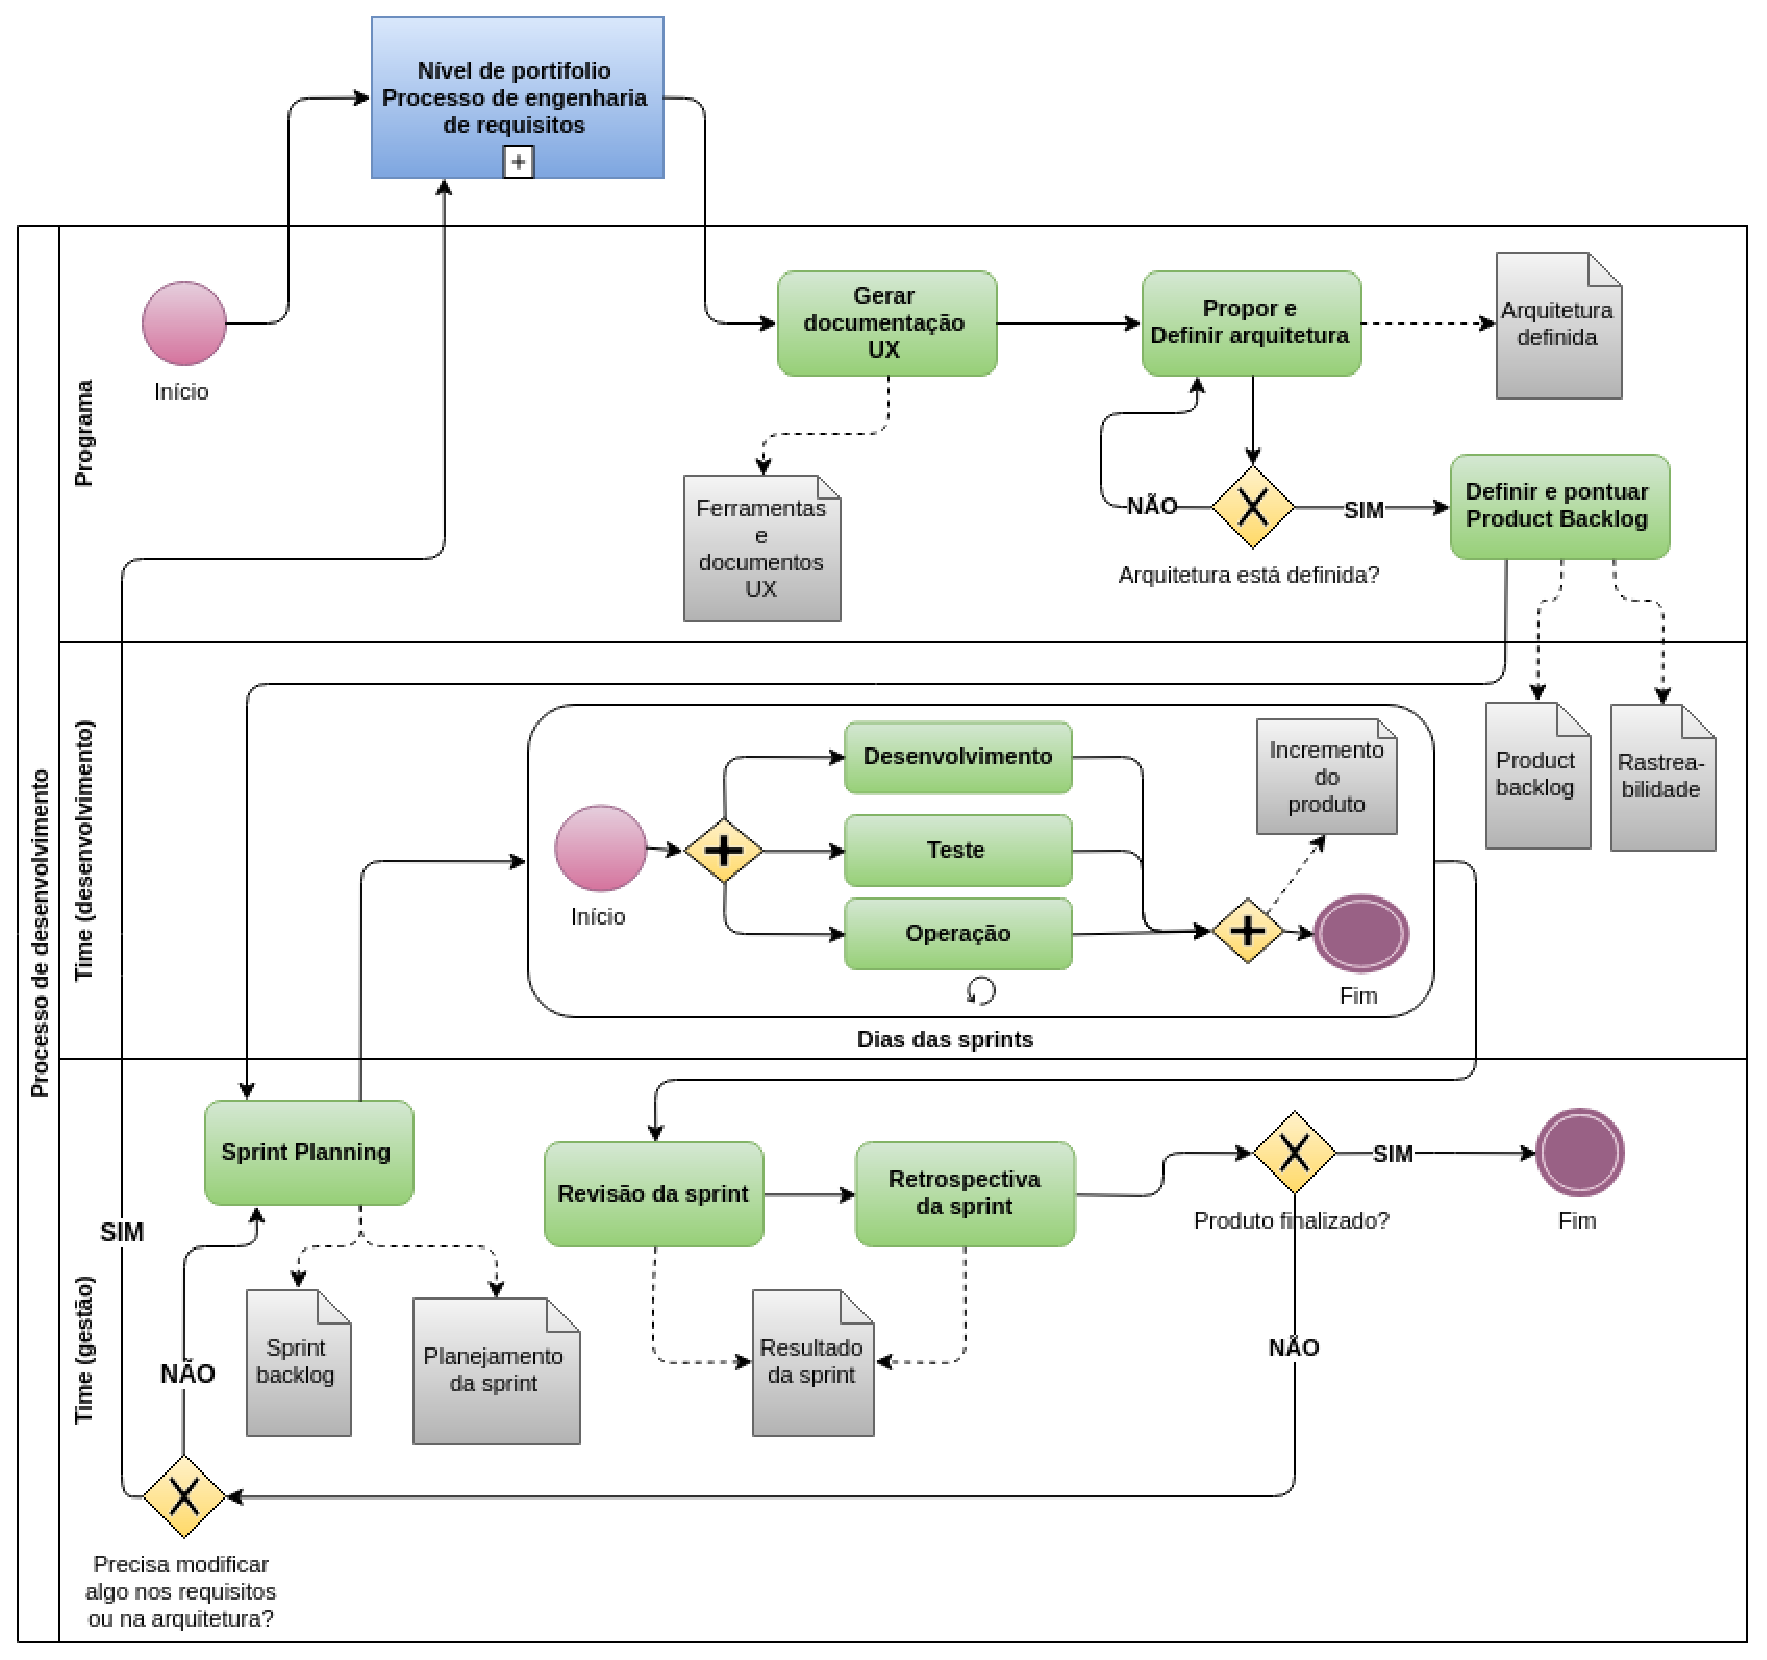
\includegraphics[keepaspectratio=true,scale=0.5]{figuras/desenvolvimento.eps}
  \caption[Processo de desenvolvimento.]{Processo de desenvolvimento. Fonte: Autor}
	\label{fig:desenvolvimento}
\end{figure}

\subsection{Nível de Portfólio}

Dentro da Engenharia de Software vários modelos definem as etapas necessárias para se construir um software de acordo com o processo definido, mas todos têm algo em comum: uma etapa dedicada a compreensão dos problemas a serem solucionados e a definição do quê será feito. Esta etapa inicial recebe o nome de engenharia de requisitos e está localizado no nível de portfólio do SAFe \cite{pressman}.

O nível de portfólio definido para a etapa de engenharia de requisitos do software PGTBL segue três
fases principais:

\subsubsection{Elicitação}

Em paralelo ao processo do TCC o processo de desenvolvimento se inicia com o subprocesso de engenharia de requisitos na
parte de elicitação.

Essa atividade preocupa-se com o levantamento dos principais aspectos, sejam eles funcionais e/ou não funcionais.
Podemos dizer que passamos de um alto nível de abstração para algo mais próximo do mundo real utilizando várias técnicas
de elicitação. Ela se iniciou com a identificação do problema e o contexto na qual o software foi aplicado, além definir
o tema de investimento. É nessa fase que é identificado os épicos (requisitos funcionais) e enables (requisitos não
funcionais) através de técnicas de elicitação como brainstorms e prototipação. Com isso os épicos (EP) são separados em
pedaços menores chamados Features (EN).

\subsubsection{Modelagem}

Na fase de modelagem objetiva-se criar um modelo organizacional em contexto com o uso do software, diagramas que auxilia
na construção das funcionalidades por meio da modelagem UML, por exemplo, diagrama de classe, além de criar a modelagem
do banco de dados relacional utilizando a modelo entidade relacionamento (MER). Na parte não funcional foi criado
diagramas que auxilia a identificação e rastreabilidade de requisitos não funcionais como metas a serem alcançadas
através do framework NFR.

\subsubsection{Análise}

Na fase de análise objetiva-se criar todos os documentos relacionados ao gerenciamento do projeto, por exemplo,
documento de abertura de projeto, plano de gerenciamento de recursos humanos, comunicação, risco, medição e análise,
configuração de software, aquisição e custos. Além disso nessa fase foi elaborado o documento de visão do projeto.

\subsection{Nível de Programa}

Nível responsável pela auto-organização de times ágeis, entrega contínua de valor, criação de Features por meio dos épicos encontrados, realização de toda a documentação relacionada ao \textit{User Experience} ou UX, e definição do documento de arquitetura do software.


No nível de programa foi definido a arquitetura que melhor se adapte ao projeto, utilizaremos de algumas técnicas de UX
e UI para melhorar a usabilidade do software e foi elaborado e pontuado as histórias de usuário do product backlog,
essas foram derivadas das features definidas no nível de portfólio.

\subsection{Nível de Time}

Nível responsável pelo auto-gerenciamento da equipe ágil, incremento do software totalmente testado, práticas SCRUM e XP, descrição do valor por meio de histórias de usuário e tarefas.

O nível de time se inicia com a \textit{Sprint Planning}, na qual será priorizada as histórias de usuário que serão implementadas na \textit{sprint} que se segue. Com isso inicia-se os ciclos de desenvolvimento das sprints. Dentro dessa atividade temos em paralelo o desenvolvimento, teste e operações (DevOps) tendo como resultado o incremento do produto.

Ao finalizar o ciclo de desenvolvimento será realizado a revisão da sprint, em que será apresentado as funcionalidades implementadas e verificar se há alguma dívida técnica para a próxima iteração que se segue. Em seguida será realizada a retrospectiva da sprint que será coletado pontos positivos, negativos e melhorias para as próximas iterações.

Todo o processo foi executado de forma iterativa e incremental, ou seja, a cada iteração chamada de sprint, foi retomado e avaliado se houve necessidade de alguma modificação ou incremento nesses diagramas e documentos. Além de que na finalização de cada fase teve uma atividade de revisão dos documentos e em paralelo com todo o processo teve o processo de medição e análise responsável pela coleta de métricas de qualidade.
